SSD采用了多尺度的特征图进行检测,这不同于YOLO算法,其基本架构如图\ref{ssd}所示。
\begin{uscfigure}
	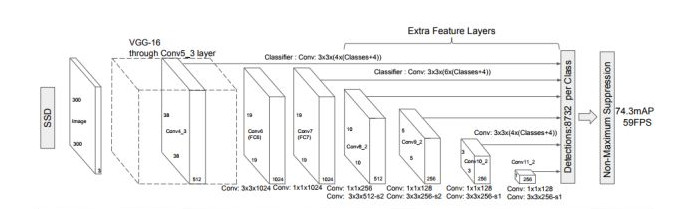
\includegraphics[width=\textwidth]{./Pictures/ssd_model.jpg}	
	\caption{SSD基本框架}
	\label{ssd}
\end{uscfigure}


概括地可以将SSD算法的核心思想归结为以下三点

\textbf{1、采用多尺度特征图用于检测 }

所谓多尺度,即采用大小不同的特征图用于检测,如图\ref{multiscale}所示,一般前面的CNN网络其特征图会比较大,后面会采用步长为的卷积或者池化的方式来缩小特征图的大小,
\begin{uscfigure}
	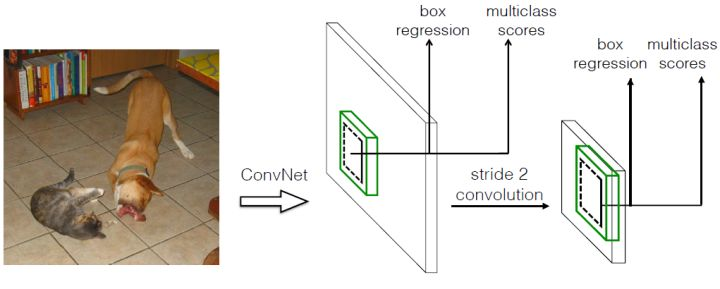
\includegraphics[width=\textwidth]{./Pictures/ssd_(1).jpg}	
	\caption{采用多尺度用于检测}
	\label{multiscale}
\end{uscfigure}
不同尺度下得到用来做的特征图都被检测。如图\ref{featuremap}所示,8x8的特征图可以被划分为更多的单元,但是得到的每个单元的先验框尺度比较小。这样做的优点是相对较小的目标用比较大的特征图来检测,相对较大的目标用小的特征图来检测。
\begin{uscfigure}
	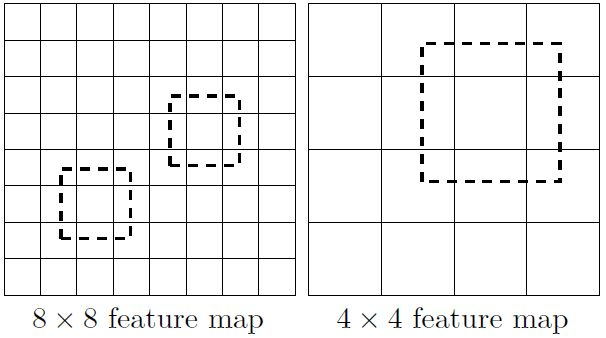
\includegraphics[width=\textwidth]{./Pictures/ssd_(2).jpg}	
	\caption{8x8与4x4的特征图}
	\label{featuremap}
\end{uscfigure}

\textbf{2、采用卷积进行检测}

SSD算法直接采用卷积对不同的特征图进行提取检测结果。采用$ 3\times 3 \times p $这样比较小的卷积核就可以得到形状为 $m\times n \times p $的特征图的检测值。 

\textbf{3、设置先验框 }

SSD算法引用了Faster R-CNN中anchor的思想,每个单元设置长宽比、大小不同的先验框一般情况下,每个单元会设置多个先验框,其尺度和长宽比存在差异,,预测的边界框(bounding boxes)是以这些先验框为基准的,在一定程度上减少训练难度。如图\ref{ssd_anchor}所示,图片中狗和猫分别采用最适合它们形状的先验框来进行训练,可以看到每个单元使用了4个不同的先验框,后面会详细讲解训练过程中的先验框匹配原则。
\begin{uscfigure}
	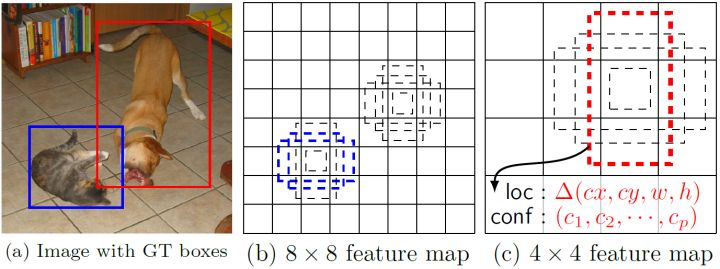
\includegraphics[width=\textwidth]{./Pictures/ssd_(3).jpg}	
	\caption{SSD算法中的先验框}
	\label{ssd_anchor}
\end{uscfigure}